
\section{Teacher Student Capacity Gaps}
\label{sec:teacher-student-capacity-gaps}

In this section, we examine the capacity gap in two settings: kernel regression and a synthetic example using \gls{mlp} for a mapping problem. The kernel regression setup provides a theoretical and analytically tractable perspective on the capacity gap. The \gls{mlp}-based synthetic example allows us to study the capacity gap in a more practical, learnable function approximation scenario. By analyzing these two setups, we aim to better understand the fundamental limitations of distillation when there is a significant mismatch between teacher and student capacities.

\subsection{Kernel Regression}
\label{ssec:kernel-regression}
One of our main contributions is that the student loss follows a broken power law, where the transition between the two power law regions 
occur when the student becomes a stronger learner than the
teacher (\Cref{eq:distillation-scaling-law}). 
This implies that making the teacher too capable (relative to the student)
reduces student performance.
In this section we show how a capacity gap provably degrades student performance in the setting of kernel regression. 
While simple, we believe the underlying principle causing the student performance degradation in this case carry over to much more general settings involving neural networks.
\subsubsection{Setup}
\label{sssec:setup}
Let $\mathcal{H}$ denote a Hilbert space spanned by orthonormal bases functions 
$\{\phi_i\}_{i=1}^\infty$ 
such that $\langle \phi_i,\phi_j \rangle_{\mathcal{H}} = \delta_{ij}$. 
Let $f^* \in \mathcal{H}$ denote the \emph{target function}, identified by a set of coefficients $\bm{\alpha} = \{\alpha_i\}_{i=1}^\infty \in \R,~\|\alpha\| = M<\infty$ such that:
\begin{align}
	f^\star(x) = \sum_{i=1}^\infty \alpha_i\phi_i(x).
\end{align}
Let $\mathcal{H}_t^m,\mathcal{H}_s^n$ denote the teacher and student Hilbert spaces respectively:
\begin{align}
	\mathcal{H}_t^m & = \text{Span}\{\phi_1,\phi_2,...,\phi_m\}, \\
	\mathcal{H}_s^n & = \text{Span}\{\phi_1,\phi_2,...,\phi_n\},
\end{align}
which are the hypothesis spaces of the teacher and student.
Note that while the Hilbert space $\mathcal{H}$ is spanned by an infinite orthonormal basis, the teacher and student spaces are \emph{finite} and spanned by $m$ and $n$ basis functions respectively, where $|m-n|$ represents the teacher and student capacity gap. 

The process of training the teacher and student models involves solving the following constrained optimization problems:
\begin{align}
	g^\star & = \min_{g \in \mathcal{H}_t^m}\|g - f^\star\|_\mathcal{H} ~~~\text{s.t}~~~ \|g\|_\mathcal{H} \leq T, \\
	h^\star & = \min_{h \in \mathcal{H}_s^n}\|h - g^\star\|_\mathcal{H} ~~~\text{s.t}~~~ \|h\|_\mathcal{H} \leq D,
\end{align}
where $g^\star, h^\star$ are the optimal teacher and student respectively, and $D\leq T<M$. Note that we assume the teacher and student are exposed to an infinite amount of training data, hence our analysis is carried over entirely in function space.

\begin{lemma}\label{lem:teacher}
	The optimal teacher $g^\star$ is given by:
	\begin{align}\label{eqn:c}
		g^\star(x) = C(m,T)\sum_{i=1}^m\alpha_i \phi_i(x),~~~C(m,T) = \begin{cases}
			                                                              1                                       & \sqrt{\sum_{i=1}^m\alpha_i^2}\leq T \\
			                                                              \frac{T}{\sqrt{\sum_{i=1}^m\alpha_i^2}} & \text{otherwise.}
		                                                              \end{cases}
	\end{align}
	The teacher error $e^\star_\text{teacher}(m,T)$ is given by:
	\begin{align}
		e^\star_\text{teacher}(m,T) = \|g^\star - f^\star\|_\mathcal{H} = \sqrt{(C(m,T) - 1)^2\sum_{i=1}^m\alpha_i^2+ \sum_{i=m+1}^\infty \alpha_i^2}.
	\end{align}
	\begin{proof}
		By construction we may assume the teacher model takes the form $g^\star = \sum_{i=1}^m \beta_i \phi_i$.
		where $\sqrt{\sum_{i=1}^m\beta_i^2} \leq T$. We can write the error of $g^\star$ using:
		\begin{align}
			e_\text{teacher}(m,T, \bm{\beta}) & = \Big\|\big(\sum_{i=1}^m(\beta_i - \alpha_i)\phi_i + \sum_{i=m+1}^\infty \alpha_i\phi_i\Big\|_\mathcal{H}  = \sqrt{\sum_{i=1}^m(\beta_i - \alpha_i)^2 + \sum_{i=m+1}^\infty \alpha_i^2 }.\label{eqn:min}
		\end{align}
		Note that the minimizing coefficients $\bm{\beta}^\star$ of \cref{eqn:min} must take the form $\bm{\beta} = C\bm{\alpha}$ for some coefficient $C$. Considering the norm constraint on $g$, the constant $C$ takes the form in \cref{eqn:c}. Plugging the resulting $g^\star$ into the expression for $e_\text{teacher}(m,T, \bm{\beta}^\star)$ completes the proof.
	\end{proof}
\end{lemma}

Notably and intuitively, the teacher error decreases monotonically as $m$, which represents the teacher model capacity, increases.
\subsubsection{Distilling the Teacher}
\label{sssec:distilling-the-teacher}

We now pick our student function $h^\star$ by mimicking the teacher subject to a norm constraint:
\begin{align}
	h^\star(x) = \min_{h \in \mathcal{H}_t^n}\|h - g^\star\|_\mathcal{H} ~~~\text{s.t.}~~~ \|h\|_\mathcal{H} \leq D.
\end{align}
\begin{lemma}\label{lem:student}
	Let $k = \min(m,n)$ be the smaller of the teacher and student capacities. The optimal student $h^\star$ is given by:
	\begin{align}
		h^\star    & = Q(m,k,T,D)C(m,T)\sum_{i=1}^k\alpha_i\phi_i            \\
		Q(m,k,T,D) & = \begin{cases}
			               1                                             & C(m,T)\sqrt{\sum_{i=1}^k\alpha_i^2}<D \\
			               \frac{D}{C(m,T)\sqrt{\sum_{i=1}^k\alpha_i^2}} & \text{otherwise.}
		               \end{cases} \label{eqn:q}
	\end{align}
	The student error with respect to the target function is then:
	\begin{align}
		e_\text{student}(m,n,T,D) = \|h^\star - f^\star\|_\mathcal{H} = \sqrt{(C(m,T)Q(m,k,T,D) - 1)^2\sum_{i=1}^k\alpha_i^2+ \sum_{i=k+1}^\infty \alpha_i^2}
	\end{align}
	\begin{proof}
		The proof follows the exact same logic as in \cref{lem:teacher}. i.e, we can assume the optimal student is given by $h^\star = \sum_{i=1}^n \gamma_i \phi_i$. From the distillation loss, the optimal coefficients must match the teacher coefficients for the basis functions $\{\phi_i\}_{i=1}^n$, perhaps rescaled due to the norm constraint $\sqrt{\sum_{i=1}^n \gamma_i^2}\leq D$. This rescaling then gives rise to the additional $Q(m,k,T,D)$ multiplier in \cref{eqn:q}.
	\end{proof}
\end{lemma}

\subsubsection{U-shape in the student error}
\label{sssec:u-shape-in-the-student-error}

We will prove that the map
\[
	m \;\longmapsto\; e_{\text{student}}(m,n,T,D)
\]
is comprised of two distinct segments: i) where the student error monotonically decreases for $m < n$, and ii) where it monotonically increases for $m \geq n$, establishing a U-shape in the student error echoing the trend seen in \cref{fig:isoflop-teacher-fixedm-students,fig:fixedm-teacher-fixedm-students}.

\medskip

\noindent
\textbf{Case 1: $m < n$. \, (Student error is non-increasing in $\bm m$)}
\smallskip

\noindent
\emph{Claim.} For $1 \le m < n$, we have
\[
	e_{\text{student}}(m+1,n,T,D)
	\;\;\le\;\;
	e_{\text{student}}(m,n,T,D). \label{claim:1}
\]
In words, when $m < n$, the error does not increase (and typically decreases) as the teacher capacity $m$ increases.

\noindent
\emph{Proof.}

Let $\mathcal{H}_t^{m,T} \subseteq \mathcal{H}_t^{m}$ denote the space of functions in $\mathcal{H}_t^{m}$ that are norm constrained by $D$. i.e:
\begin{align}
	\mathcal{H}_t^{m,T} = \{f \in \mathcal{H}_t^{m} ~:~\|f\|_\mathcal{H}\leq T\}.
\end{align}
Since $\mathcal{H}_t^{m,T} \subseteq \mathcal{H}_t^{m+1,T}$, it follows that $g^\star_m \in \mathcal{H}_t^{m+1,T}$, which implies that the teacher error cannot increase as $m$ increases, hence it monotonically decreases. Now, let $h^\star_m$ denote the optimal student given the teacher $g^\star_m$. Since $D\leq T$, then for any $m < n$, we can equivalently write the optimal student $h^\star_m$ as the solution to the following optimization problem:
\begin{align}
	\forall_{m \leq n}~h^{\star}_m & = \min_{h \in \mathcal{H}_s^n}\|h - g^\star_m\|_\mathcal{H} ~~~\text{s.t}~~~ \|h\|_\mathcal{H} \leq D \\
	                               & = \min_{h \in \mathcal{H}_t^m}\|h - f^\star\|_\mathcal{H} ~~~\text{s.t}~~~ \|h\|_\mathcal{H} \leq D,
\end{align}
which corresponds exactly to the objective of finding the optimal teacher with with a norm constraint set to $D$. Therefore, from the fact that the teacher error monotonically decreases we can conclude that the student error monotonically decreases as well in the regime $m< n$.


\medskip

\noindent
\textbf{Case 2: $m \geq n$. \, (Student error eventually increases in $\bm m$)}

\smallskip

\noindent
\emph{Claim.} For $m \geq n$:
\[
	e_{\text{student}}(m+1,n,T,D)
	\;\;\ge\;\;
	e_{\text{student}}(m,n,T,D).
\]
Hence once $m$ exceeds $n$ the student error cannot decrease any further, the error eventually starts to rise.

\noindent
\emph{Proof.}

Let $\bm{\beta}^\star_m = \{\beta_1,...,\beta_m\}$ denote the coefficients of the optimal teacher $g^\star_m$. Note that in the regime $m\geq n$, as long as $\sqrt{\sum_{i=1}^n\beta_i^2}\geq D$ (i.e the norm of the coefficients corresponding to the basis $\{\phi_1,...,\phi_n\}$ is smaller than $D$), we have from \cref{eqn:q} that $Q(m,k,T,D) = 1$, which means that the optimal student doesnt change, hence its error remains constant. If however $\sqrt{\sum_{i=1}^n\beta_i^2}<D$, then we have from \cref{eqn:q}:
\begin{align}
	1 > Q(m,k,T,D) \geq Q(m+1,k,T,D),
\end{align}
where the second inequality becomes strict if $\alpha_{m+1}^2>0$. A strict inequality (i.e $Q(m,k,T,D) > Q(m+1,k,T,D)$) implies the optimal student is further scaled down due to the teacher having to "spread its capacity" to additional basis functions that are not learnable by the student, thereby strictly increasing its error.
Hence for $m\geq n$, we get
\[
	e_{\text{student}}(m+1,n,T,D)
	\;\;\ge\;\;
	e_{\text{student}}(m,n,T,D),
\]
demonstrating that the error increases monotonically with $m$ once $m\geq n$.
\qed

\medskip

\noindent
\textbf{Conclusion (U-shaped trend).} Combining these two cases:
\[
	\begin{cases}
		\text{For }1 \le m < n: &
		e_{\text{student}}(m,n,T,D)\text{ monotonically decreasing in }m, \\[4pt]
		\text{For }m\geq n:     &
		e_{\text{student}}(m,n,T,D)\text{ monotonically increasing in }m.
	\end{cases}
\]
Therefore, as a function of $m$, the student error $e_{\text{student}}(m,n,T,D)$
\emph{first decreases} and \emph{then increases} (for $m\geq n$) (for $m\le n$), giving a u-shape in student error due to a capacity gap between the teacher and the student.
\hfill\qedsymbol

We present an empirical verification of these conclusions in \Cref{fig:kernel}.

\begin{figure}[h]
	\centering
	\includegraphics[width=0.3\textwidth]{plots/kernel_error_v2.pdf}
	\caption{\textbf{Distillation in kernel regression.} We randomly sample the $\bf{\alpha} = \{\alpha_1,...,\alpha_{1000}\}$ coefficients of the target function uniformly in the range $[-1,1]$. We fix $T = 5, D = 4.5$ and compute the optimal student and teacher errors according to \cref{lem:teacher,lem:student} for various values of $n$ (dashed curves), and for $m \in [1...1000]$. As can be seen, the student error exhibits a U shaped error curve as predicted by the theory, where the error starts to increase when $m\geq n$. The black solid line indicates the teacher error, which always decreases with increasing $m$.}
    \label{fig:kernel}
\end{figure}
The above theoretical analysis points to an intuitive interpretation of the potentially adverse effect of a large teacher-student capacity gap; the degradation in student performance is due to the teacher learning basis functions that are unreachable by the student, at the expense of basis functions that are reachable by the student. In the following we provide empirical evidence in support of this picture in a controlled yet more realistic setting.

\FloatBarrier
\subsection{MLPs on the Mapping Problem}
\label{ssec:mlps-on-the-mapping-problem}

\subsubsection{Problem Definition}
\label{sssec:problem-definition}

Here we show a synthetic setting which exhibits the U-shape phenomenon. 
Matching the kernel regression analysis (\Cref{ssec:kernel-regression}), 
we find that the synthetic problem must include a class of problems that are easy for the student to learn, and ones that are harder, in order for the u-shape to appear.

The problem setting is the \emph{Mapping Problem}, and is 
similar in spirit to Pointer Value Retrieval \citep{DBLP:journals/corr/abs-2107-12580},
Here, the input is composed of small integers in \{0,1,2\}. 
The label for each sample is given by the code below, which shows the two cases: i) one where the label is simply given by a one-hot position, and ii) one where the label is given by the location of a matching element in the context portion of the input.  

\begin{minipage}{.6\textwidth}
	This Section comprehensively catalogs the potential applications of MU to assist AIA compliance. 
% In creating this catalog, we make a distinction between MU for system- and model-centered requirements like those in \citep[Art. 9, 15, 53, 55]{european_union_ai_act_2024} and MU for data-centered requirements like those in \citep[Art. 10]{european_union_ai_act_2024}. 
For each, we analyze the SOTA and its ability to support the potential application, then identify any open questions the research community must resolve in order to bridge the gap between the two. 
% \subsection{MU to aid compliance with system- and model-centered AIA requirements}
 % Some AIA provisions require AI systems or GPAI models, at large, to satisfy certain criteria --- e.g., related to risk mitigation \citep[Arts. 9, 55]{european_union_ai_act_2024}, accuracy and cybersecurity \citep[Art. 15]{european_union_ai_act_2024}, or copyright law \citep[Art. 53]{european_union_ai_act_2024}. When problematic training data points (i.e., the forget set) are what is holding the system or model back from achieving these criteria, and where MU, by diminishing the impact of those data points in an already-trained model, can help the system or model achieve the decreed criteria, it seems reasonable to hypothesize that MU can be a viable tool for compliance with these particular provisions.
 % One potential snag here might involve problematic training data points that also happen to violate requirements of the AIA (notably, those of Article 10). Are all downstream models trained on those data points ``poisoned fruit'' that are irredeemably non-compliant themselves, regardless of any post-training adjustments like approximate MU (or fine-tuning) that do not retrain without the problematic data? Though we assume for the remainder of this section that this is not the case, it is among the points that we ask legislators or standard-setters\footnote{The AIA \citep[Art. 40]{european_union_ai_act_2024}, like other EU product regulation, relies heavily on harmonised standards, which are detailed technical solutions prepared by the EU's external standardisation organisations (CEN, CENELEC and ETSI) and which, if complied with by the regulated entities, ``have the legal effect of establishing a presumption of conformity'' with the relevant requirements \citep{mazzini2023proposal}} to clarify.
In sum, we find that the potential applications of MU to assist AIA compliance ultimately roll up into just six separate applications (Fig. \ref{fig:pyramids}):
\begin{itemize}[noitemsep, topsep=0pt]
    \item Improve accuracy per \citet[Arts. 9, 15]{european_union_ai_act_2024}; 
    \item Mitigate bias per \citet[Arts. 9, 55]{european_union_ai_act_2024}; 
    \item Mitigate confidentiality attacks per \citet[Arts. 9, 15, 55]{european_union_ai_act_2024}); 
    \item Mitigate data poisoning per \citet[Arts. 15]{european_union_ai_act_2024}); 
    \item Mitigate other risks of generative outputs per \citet[Arts. 9, 55]{european_union_ai_act_2024}); 
    \item Aid compliance with copyright laws, per \citet[Art. 53]{european_union_ai_act_2024})
\end{itemize}

\begin{figure*}[ht]

\begin{center}

\scalebox{0.6}{





\tikzset{every picture/.style={line width=0.75pt}} %set default line width to 0.75pt        

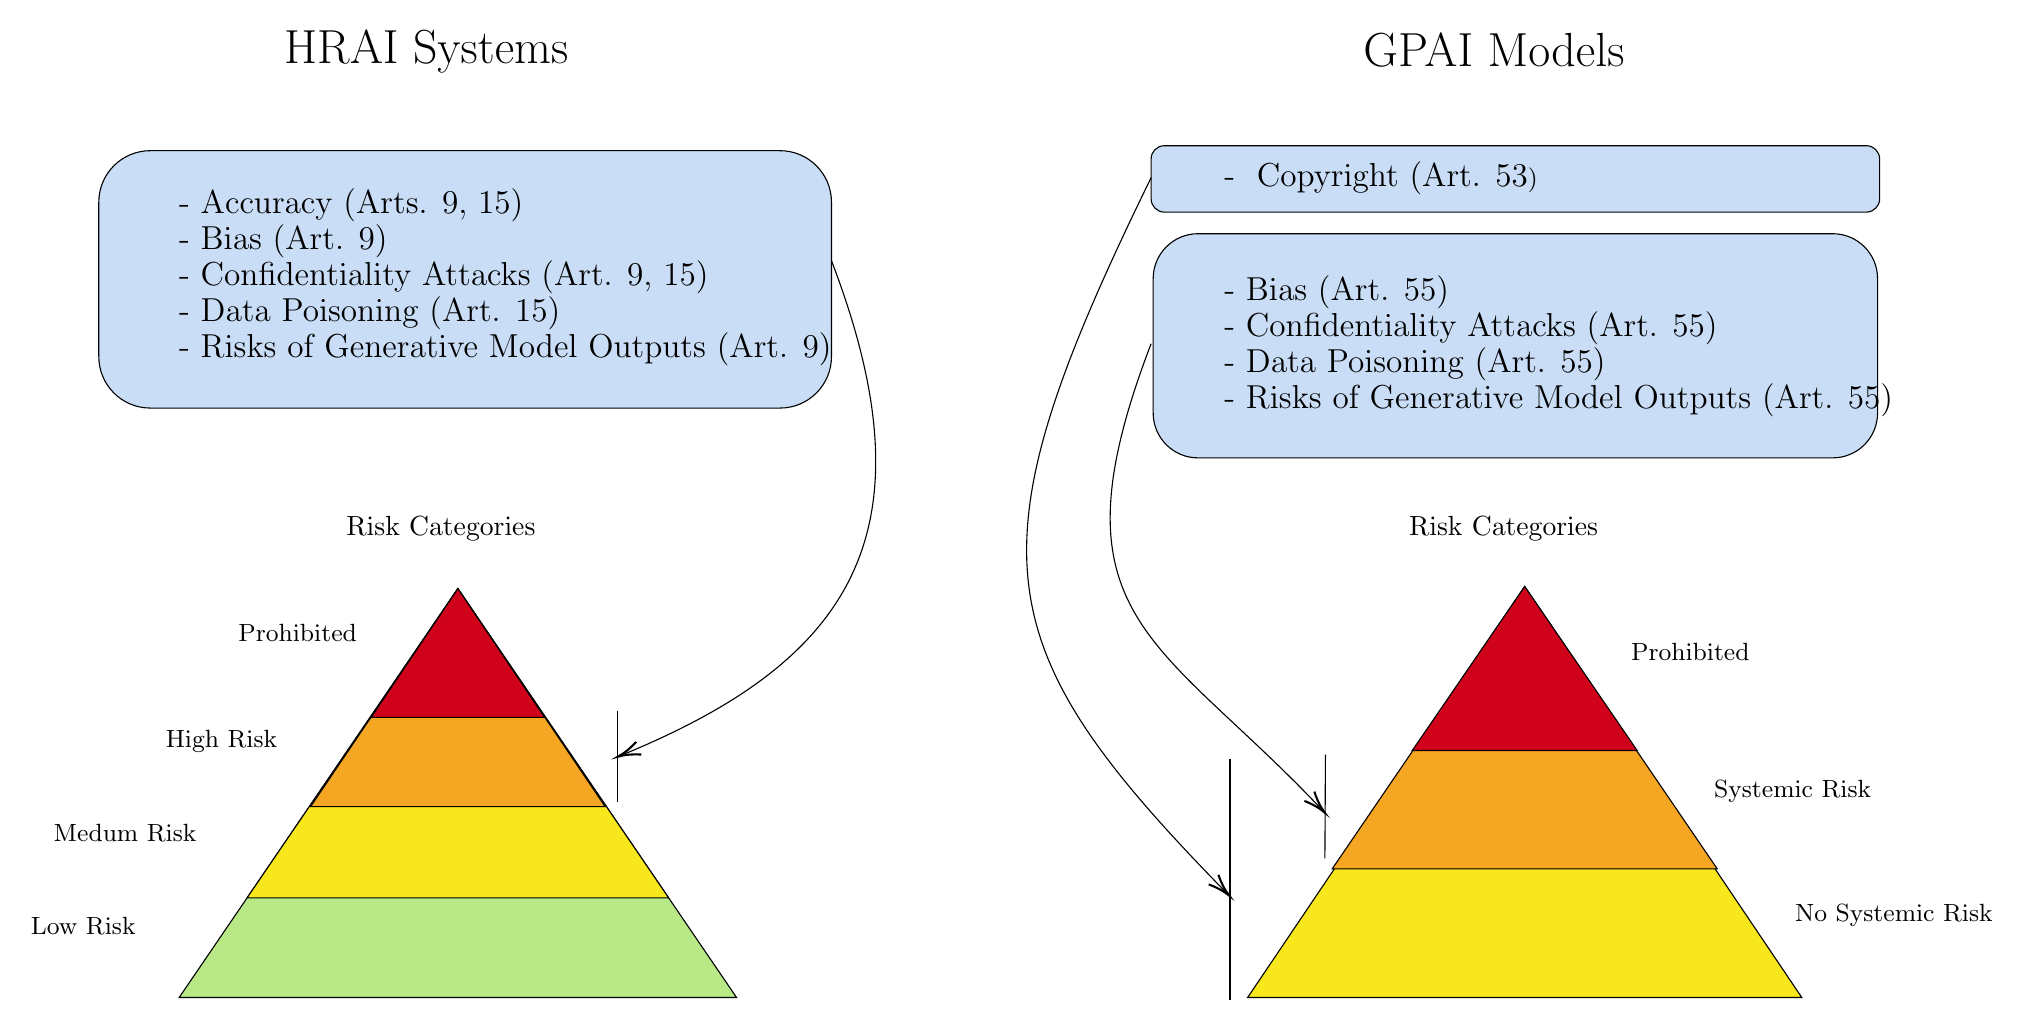
\begin{tikzpicture}[x=0.75pt,y=0.75pt,yscale=-1,xscale=1]
%uncomment if require: \path (0,592); %set diagram left start at 0, and has height of 592

%Shape: Triangle [id:dp5428005874858406] 
\draw  [fill={rgb, 255:red, 184; green, 233; blue, 134 }  ,fill opacity=1 ] (234,341) -- (368.28,538) -- (99.72,538) -- cycle ;
%Shape: Triangle [id:dp3047849031551493] 
\draw  [fill={rgb, 255:red, 248; green, 231; blue, 28 }  ,fill opacity=1 ] (748,340) -- (881.5,538) -- (614.5,538) -- cycle ;
%Shape: Triangle [id:dp0818620622382471] 
\draw  [fill={rgb, 255:red, 245; green, 166; blue, 35 }  ,fill opacity=1 ] (748,340) -- (840.75,476) -- (655.25,476) -- cycle ;
%Shape: Triangle [id:dp7631457704181537] 
\draw  [fill={rgb, 255:red, 208; green, 2; blue, 27 }  ,fill opacity=1 ] (748,340) -- (802.19,419) -- (693.81,419) -- cycle ;
%Shape: Triangle [id:dp7055596435513258] 
\draw  [fill={rgb, 255:red, 248; green, 231; blue, 28 }  ,fill opacity=1 ] (234,341) -- (335.56,490) -- (132.44,490) -- cycle ;
%Shape: Triangle [id:dp9202964178531197] 
\draw  [fill={rgb, 255:red, 245; green, 166; blue, 35 }  ,fill opacity=1 ] (234,341) -- (304.94,446) -- (163.06,446) -- cycle ;
%Shape: Triangle [id:dp09535399425331859] 
\draw  [fill={rgb, 255:red, 208; green, 2; blue, 27 }  ,fill opacity=1 ] (234,341) -- (275.77,403) -- (192.23,403) -- cycle ;
%Rounded Rect [id:dp25406852669435454] 
\draw  [fill={rgb, 255:red, 201; green, 221; blue, 246 }  ,fill opacity=1 ] (61,154.8) .. controls (61,141.1) and (72.1,130) .. (85.8,130) -- (389.2,130) .. controls (402.9,130) and (414,141.1) .. (414,154.8) -- (414,229.2) .. controls (414,242.9) and (402.9,254) .. (389.2,254) -- (85.8,254) .. controls (72.1,254) and (61,242.9) .. (61,229.2) -- cycle ;
%Rounded Rect [id:dp6638236112064699] 
\draw  [fill={rgb, 255:red, 201; green, 221; blue, 246 }  ,fill opacity=1 ] (569,191.6) .. controls (569,179.67) and (578.67,170) .. (590.6,170) -- (896.4,170) .. controls (908.33,170) and (918,179.67) .. (918,191.6) -- (918,256.4) .. controls (918,268.33) and (908.33,278) .. (896.4,278) -- (590.6,278) .. controls (578.67,278) and (569,268.33) .. (569,256.4) -- cycle ;
%Curve Lines [id:da6560168607616261] 
\draw    (414,183) .. controls (464.75,315.34) and (422.43,376.39) .. (312.66,421.32) ;
\draw [shift={(311,422)}, rotate = 337.93] [color={rgb, 255:red, 0; green, 0; blue, 0 }  ][line width=0.75]    (10.93,-3.29) .. controls (6.95,-1.4) and (3.31,-0.3) .. (0,0) .. controls (3.31,0.3) and (6.95,1.4) .. (10.93,3.29)   ;
%Straight Lines [id:da5242356218911126] 
\draw    (311,400) -- (311,444) ;
%Rounded Rect [id:dp6795269102209953] 
\draw  [fill={rgb, 255:red, 201; green, 221; blue, 246 }  ,fill opacity=1 ] (568,134) .. controls (568,130.47) and (570.87,127.6) .. (574.4,127.6) -- (912.6,127.6) .. controls (916.13,127.6) and (919,130.47) .. (919,134) -- (919,153.2) .. controls (919,156.73) and (916.13,159.6) .. (912.6,159.6) -- (574.4,159.6) .. controls (570.87,159.6) and (568,156.73) .. (568,153.2) -- cycle ;
%Straight Lines [id:da5998648988158835] 
\draw    (606,423) -- (606,539) ;
%Curve Lines [id:da489843699645353] 
\draw    (568,223) .. controls (517.26,355.34) and (571.45,363.92) .. (650.54,447.73) ;
\draw [shift={(651.73,449)}, rotate = 226.83] [color={rgb, 255:red, 0; green, 0; blue, 0 }  ][line width=0.75]    (10.93,-3.29) .. controls (6.95,-1.4) and (3.31,-0.3) .. (0,0) .. controls (3.31,0.3) and (6.95,1.4) .. (10.93,3.29)   ;
%Straight Lines [id:da4800745204547854] 
\draw    (652,421) -- (651.73,471) ;
%Curve Lines [id:da31844169520160337] 
\draw    (568,143) .. controls (479,325) and (487,368) .. (605.73,489) ;
\draw [shift={(605.73,489)}, rotate = 225.54] [color={rgb, 255:red, 0; green, 0; blue, 0 }  ][line width=0.75]    (10.93,-3.29) .. controls (6.95,-1.4) and (3.31,-0.3) .. (0,0) .. controls (3.31,0.3) and (6.95,1.4) .. (10.93,3.29)   ;

% Text Node
\draw (691,305) node [anchor=north west][inner sep=0.75pt]  [font=\normalsize] [align=left] {Risk Categories};
% Text Node
\draw (798,366) node [anchor=north west][inner sep=0.75pt]  [font=\small] [align=left] {Prohibited};
% Text Node
\draw (838,432) node [anchor=north west][inner sep=0.75pt]  [font=\small] [align=left] {Systemic Risk};
% Text Node
\draw (877,492) node [anchor=north west][inner sep=0.75pt]  [font=\small] [align=left] {No Systemic Risk};
% Text Node
\draw (179,305) node [anchor=north west][inner sep=0.75pt]  [font=\normalsize] [align=left] {Risk Categories};
% Text Node
\draw (127,357) node [anchor=north west][inner sep=0.75pt]  [font=\small] [align=left] {Prohibited};
% Text Node
\draw (92,408) node [anchor=north west][inner sep=0.75pt]  [font=\small] [align=left] {High Risk};
% Text Node
\draw (27,498) node [anchor=north west][inner sep=0.75pt]  [font=\small] [align=left] {Low Risk};
% Text Node
\draw (38,453) node [anchor=north west][inner sep=0.75pt]  [font=\small] [align=left] {Medum Risk};
% Text Node
\draw (98.4,147) node [anchor=north west][inner sep=0.75pt]  [font=\scriptsize] [align=left] {{\large - Accuracy (Arts. 9, 15)}\\{\large - Bias (Art. 9)}\\{\large - Confidentiality Attacks (Art. 9, 15)}\\{\large - Data Poisoning (Art. 15)}\\{\large - Risks of Generative Model Outputs (Art. 9)}};
% Text Node
\draw (602,189) node [anchor=north west][inner sep=0.75pt]  [font=\scriptsize] [align=left] {{\large - Bias (Art. 55)}\\{\large - Confidentiality Attacks (Art. 55)}\\{\large - Data Poisoning (Art. 55)}\\{\large - Risks of Generative Model Outputs (Art. 55)}};
% Text Node
\draw (149,71) node [anchor=north west][inner sep=0.75pt]  [font=\LARGE] [align=left] {HRAI Systems};
% Text Node
\draw (669,72) node [anchor=north west][inner sep=0.75pt]  [font=\LARGE] [align=left] {GPAI Models};
% Text Node
\draw (602.03,134) node [anchor=north west][inner sep=0.75pt]  [font=\scriptsize] [align=left] {{\large - \ Copyright (Art. 53}{\small )}};


\end{tikzpicture}

}

\end{center}
\caption{\textit{\textbf{AIA Uses Cases for Machine Unlearning.}}\label{fig:pyramids}}
\end{figure*}

 % In the meantime, we explore the application of MU to aid compliance with six system- and model-centered AIA requirements: (1) risk mitigation of risks to health and safety in AI models (2) 
 
 % Meanwhile, MU is a process for altering the behavior of an already-trained model (so that it behaves the same as a model that was not trained on the forget set) \cite{Xu_2024}. Where altering a model's behavior in this manner helps it (or the AI system it inhabits) satisfy the decreed criteria, MU's potential to aid compliance seems straightforward from a legal perspective (and the discussion then becomes one about technical feasibility). We argue this is the case for the AIA provisions requiring AI systems and/or GPAI models to mitigate certain risks \citep[Arts. 9, 55]{european_union_ai_act_2024}, to achieve accuracy and cybersecurity \citep[Art. 15]{european_union_ai_act_2024}, or to comply with EU copyright law \citep[Art. 53]{european_union_ai_act_2024}. 

 

\subsection{Accuracy}
\label{sssec:accuracy}

At least two AIA provisions may compel HRAI systems providers towards higher levels of accuracy. First (and most direct), HRAI systems must achieve a level of accuracy appropriate to their intended use and the SOTA \citep[Art. 15.1; Rec. 74]{european_union_ai_act_2024}. Second, HRAI systems' risk management must include measures to mitigate or eliminate risks to health and safety \citep[Art. 9]{european_union_ai_act_2024}, which could stem from low accuracy in domains like medicine \citep{jongsma2024why, james, Heaven2021}. For these requirements, MU can boost HRAI system's accuracy by removing the problematic data from the model. 

Importantly, the accuracy use case should not require privacy guarantees on the unlearned data \citep{goel2023adversarialevaluationsinexactmachine}. Rather, because the goal is strictly to boost accuracy to the level deemed appropriate  \citep[Art. 15]{european_union_ai_act_2024} or until the overall residual risk to health and safety posed by the inaccuracy is judged to be ''acceptable'' \citep[Art. 9]{european_union_ai_act_2024}, model accuracy should be the primary benchmark for MU's efficacy. In measuring that, AI providers will presumably account for any inadvertent, counteracting degradation in accuracy caused by the MU itself \cite{LI2024100254, DBLP:conf/sp/BourtouleCCJTZL21, Xu_2024}. However, providers will have to separately measure and account for the other trade-offs of using MU, such as its increased privacy and security risks \citep{Xu_2024, carlini2022privacyonioneffectmemorization}.  

% wherever doing so can ``reasonably'' be accomplished through the development or design of the system, to the point where the ''overall residual risk'' is ''judged to be acceptable'' \citep[Art. 9]{european_union_ai_act_2024}. 

% Even when limiting the definition of health and safety to physical safety, we can identify at least two scenarios where MU can serve as a ``post-training risk mitigation mechanism'' \citep{liu_unlearning_2023} that can help reduce, if not eliminate, the risks that problematic training data points can pose to health and safety. The first is where those problematic training data points --- e.g, mislabeled data points and outliers --- are leading to poor model performance that. 

% For example, incorrect labels in a training set may lead to model "confusion" and misclassification \cite{kurmanji2023unboundedmachineunlearning}. In the medical domain, misclassification can lead to patient harm and even "fatal outcomes" \citep{10.1001/jamadermatol.2023.5550}, including during diagnosis \cite{CHOWDHURY2024100297, PIRI201815, doi:10.4258/hir.2023.29.2.120} or triage \citep{saria2018better}. Because MU may help reduce confusion if the mislabeled examples are placed in the forget set \cite{kurmanji2023unboundedmachineunlearning, goel2023adversarialevaluationsinexactmachine}, we can logically conclude that MU, at least when it comes to incorrect labels in a training set, represents a viable mitigation for the risks to health and safety and, therefore, a path towards compliance with \citep[Art. 9]{european_union_ai_act_2024}. 

% \begin{tcolorbox}[colback=gray!10,colframe=black!50,title=State-of-the-Art]
\textbf{Current SOTA} Both exact or approximate unlearning theoretically offer paths towards improving model accuracy by forgetting mislabeled \citep{goel2023adversarialevaluationsinexactmachine,SUGIURA20242024DAT0002, 10.1145/3196494.3196517, chen2023unlearnwantforgetefficient, DBLP:conf/fgr/GundogduUU24}, out-of-date and outlier training data points \citep{kurmanji2023machineunlearninglearneddatabases, xu2024machineunlearningtraditionalmodels, Xu_2024, neel2024machineunlearning}, or, potentially, removing noise from medical data \citep{prelovznik2024improvingBrainMRI, dinsdale2020unlearningScannerBias}. The largest hurdle for this use case might be identifying all of the data points that are leading to inaccuracy (e.g., the mislabeled examples), which can be difficult \citep{goel2024correctivemachineunlearning}. However, for this use case, it may be good enough to identify only a subset of these examples --- so long as accuracy is boosted to levels deemed ''appropriate'' in light of the intended purpose as well as the SOTA \citep[Art. 15.1; Rec. 74]{european_union_ai_act_2024}. MU based on subset forget sets have shown success in boosting accuracy. However, other studies have suggested that you need all of polluted data, not just some of this, or it might backfire \citep{goel2024correctivemachineunlearning}. 
%For example, \citet{goel2024correctivemachineunlearning} demonstrate that the Selective Synaptic Dampening (SSD) MU technique \citep{foster2023fastmachineunlearningretraining} is able to neutralize mislabeled samples's effect on accuracy with just 10\% of mislabelled data identified. That said, SSD also fails (and, in fact, lowers overall accuracy) for the ''interclass confusion'' scenario (where sample labels samples are in correct between two classes)\citep{goel2024correctivemachineunlearning}.
%Evaluating MU success is application dependent. What's interesting here is that we probably don't need formal guarantees of unlearning the forget set here. We would probably want to see that accuracy is going up (or confusion down, etc.)
% \end{tcolorbox}
It is also important to note that evaluating unlearning success is application dependent. And, that, approximate unlearning should not be expected to yield higher accuracy than exact retraining without the low-quality data. 

\begin{tcolorbox}[colback=green!10,colframe=black!50,title=Key Points]
\begin{itemize}[leftmargin=0pt]
    \item Multiple AIA requirements may benefit from MU
    \item Theoretical guarantees may not be needed 
    \item Evaluation measure is application-dependent
\end{itemize}
\end{tcolorbox}

\vspace{1em}

\begin{tcolorbox}[colback=red!10,colframe=black!50,title=Open Problems]
\begin{itemize}[leftmargin=0pt]
    \item Lack of reliable methods for identifying problematic data to unlearn
    \item Lack of controllability over trade-offs
\end{itemize}
\end{tcolorbox}


% \subsubsection{MU to mitigate bias in HRAI systems and GPAI models with systemic risk} 
\vspace{1em}
\subsection{Bias} 

Providers of both HRAI systems and GPAI models with systemic risk may be obliged to mitigate model bias. The former must take measures to mitigate or eliminate risks to fundamental rights, which includes the right to non-discrimination \citep[Arts. 9]{european_union_ai_act_2024}). The latter must take measures to mitigate their models' systemic risk \citep[Art. 55]{european_union_ai_act_2024}, which includes the risk of large-scale discrimination \cite{gpai_code_2024}. Bias can occur because unrepresentative or incomplete data leads to model outputs that do not perform fairly on different groups or, in the case of generative models, produce stereotyped or otherwise discriminatory outputs \citep{sci6010003}. In all these cases, MU can ostensibly help forget the data points or patterns in the training set causing the bias \citep{pedregosa2023machineunlearning, neel2024machineunlearning, sai2024machineunlearning, keskpaik2024machine, chen2023unlearnwantforgetefficient, lucki2024adversarialperspectivemachineunlearning}. An important limiting factor on this use case is that training data that is not there to begin with cannot be forgotten; if the bias is due to a data \textit{deficit}, MU will not help. Because the goal here is to reduce or eradicate bias, success should ultimately be measured using traditional bias metrics like the difference in performance on various subgroups \citep{dealcala2023measuringbiasaimodels} or, in the case of generative models, the propensity for biased outputs as measured with benchmarks \citep{parrish2022bbqhandbuiltbiasbenchmark}.

% \begin{tcolorbox}[colback=gray!10,colframe=black!50,title=State-of-the-Art]
\textbf{Current SOTA}
While debiasing ML models was studied even before MU \citep{zemel2013learningfairreps}, both exact \citep{DBLP:journals/corr/abs-2405-14020}) and approximate \citep{chen2023fastmodeldebiasmachine, DBLP:conf/aistats/OesterlingMCL24, DBLP:journals/corr/abs-2405-14020}) MU have been used to mitigate model bias.
In the debiasing literature, solutions include \textit{pre-processing}, \textit{in-processing}, and \textit{post-processing} methods \citep{mehrabi2021fairnesssurvey}. MU, can mainly be considered as a post-processing method for debiasing. However, it is difficult to draw a separating line between debiasing and MU methods. MU works usually re-use some of the evaluation metrics in the debiasing literature, however, how to evaluate bias is, generally, considered an ``open problem'' \citep{reuel2024openproblemstechnicalai}. In order to preserve accuracy by not forgetting data points holistically, \citep{xu2024dontforgetmuchmachine} use MU to forget only those the features that lead to bias.

\begin{tcolorbox}[colback=green!10,colframe=black!50,title=Key Points]
\begin{itemize}[leftmargin=0pt]
    \item MU may assist compliance with multiple bias-related AIA requirements
    \item MU is only subtractive and never additive, limiting its application to this use case
        \item De-biasing solutions are not limited to MU
\end{itemize}
\end{tcolorbox}


\begin{tcolorbox}[colback=red!10,colframe=black!50,title=Open Problems]
\begin{itemize}[leftmargin=0pt]
    \item Lack of methods for identifying bias counterfactuals 
    \item  Lack of controllability over trade-offs
    \item Difficulty of guaranteeing full unlearning of biases, due to generalization
\end{itemize}
\end{tcolorbox}

% In multiple places, the AIA requires risks that have been identified to be mitigated \citep[Arts. 9.3, 55(a-b)]{european_union_ai_act_2024}. When it comes to HRAI systems, these risks include those to health and safety (including bias) and those to fundamental rights (including the right to data protection and the right to non-discrimination) \citep[Art. 9]{european_union_ai_act_2024}. When it comes to GPAI models, these risks include systemic risks \citep[Art. 55(a-b)]{european_union_ai_act_2024}. Where these risks owe to ``something undesirable'' in the training data, we know, at least as a technical matter, that MU can hypothetically serve as an effective (and economic) that reduces the relevant risk in the trained model (or, by extension, the AI system it inhabits) . 

% But does this mitigation meet the requirements of the law?
% Until further clarification by lawmakers or standard-setters, at least where the risk-causing qualities of the data do not independently violate requirements of the AIA, there is no reason to think that MU, when effective, cannot fulfill the risk mitigation requirements of \citep[Arts. 9.3, 55(a-b)]{european_union_ai_act_2024}.\footnote{Note that the same might be said of other ``post-training risk mitigation and defense mechanism[s]'' like alignment fine-tuning and content filters \citep{liu_unlearning_2023}.} Where the risk-causing qualities of the data \textit{do} independently violate requirements of the AIA (notably, those of Article 10), the picture could be more complicated. Are all downstream models the ``poisoned fruit'' of the non-compliant data and therefore irredeemably non-compliant themselves, regardless of any post-training risk mitigation techniques applied to them? Though we assume for the remainder of this section that this is not the case, it is a point that we ask legislators to clarify.
 % that can ``correct the impact of [the] bad data'' \citep{liu_unlearning_2023} and assist compliance with the relevant Act provision. 
% \subsubsection{MU to defend against confidentiality attacks on HRAI systems and GPAI models with systemic risk} 
\subsection{Confidentiality attacks} 
\vspace{-0.2cm}
The AIA requires providers of both HRAI systems and GPAI models with systemic risk to resolve and control for confidentiality attacks. Providers of HRAI systems must ensure their systems achieve an ``appropriate level'' of cybersecurity given the intended use and the SOTA, including by taking technical measures to prevent, detect, respond to, resolve and control for confidentiality attacks \citep[Art. 15.5; Rec. 74]{european_union_ai_act_2024}. Meanwhile, providers of GPAI models with systemic risk must ensure those models reflect ``an adequate level of cybersecurity'' \citep[Art. 55.d]{european_union_ai_act_2024}, which presumably also includes defending against confidentiality attacks. While the AIA does not define confidentiality attacks, we take them to include any attacks, including data reconstruction and membership inference attacks, that cause a model to reveal confidential details about its training such as data points or membership \citep{vassilev2023adversarial, CLTC2024adversarial}. This may include confidential training data memorized by generative models \citet{cooper2024machineunlearningdoesntthink, gu2024secondorderinformationmattersrevisiting, lucki2024adversarialperspectivemachineunlearning}. Where such attacks occur --- or where there is reason to think they might --- MU can ostensibly help defend against them by forgetting the confidential information vulnerable to attack \citep{hine_supporting_2024, neel2024machineunlearning, carlini2022privacyonioneffectmemorization, math12244001, xu2024machineunlearningtraditionalmodels, reuel2024openproblemstechnicalai, barez2025openproblemsmachineunlearning}.\footnote{We note that another, better solution to this problem exists: training with differential privacy (DP) \citep{Protivash_Durrell_Kifer_Ding_Zhang_2024}. Training a model with DP provides guarantees against confidentiality attacks \citep{chen2021differential, Protivash_Durrell_Kifer_Ding_Zhang_2024}. Accordingly, the safest strategy for complying with these AIA requirements is simply training with DP. We realize that this is not always practical, of course. AI providers --- for example, those integrating open source, closed-data models like Llama \citep{touvron2023llama} into their AI systems --- may only have access to the trained model weights and, therefore, training with DP is not an option. Differently, AI providers may only realize, post-training, that their model is vulnerable to confidentiality attacks and, at that point, may not be in a position to bear the cost of retraining from scratch with DP. In these situations, approximate unlearning remains a highly relevant option for addressing these attacks.} For this use case, the measure of success should be whether confidentiality attacks succeed in the wake of the MU \cite{grimes2024goneforgottenimprovedbenchmarks}, though use case-specific metrics have been developed \citet{maini2024tofutaskfictitiousunlearning}. When it comes to this use case, there are, importantly, other viable options for protecting against confidentiality attacks, including training with DP \citep{WANG2023408, kaissis2023boundingdatareconstructionattacks}.
% \begin{tcolorbox}[colback=gray!10,colframe=black!50,title=State-of-the-Art]

\textbf{Current SOTA.} Multiple techniques for using MU to mitigate confidentiality attacks (or the closely related problem of inadvertent model leakage of personal data) have been demonstrated \citep{dhingra2024protecting, ashuach2024revsunlearningsensitiveinformation, lizzo2024unlearnefficientremovalknowledge, chen2024, Wang_2024, CaoYang2015, DBLP:conf/sp/BourtouleCCJTZL21, Borkar}.
As of today, using MU to thwart these attacks can carry sizable trade-offs. For example, unlearning some data points for the sake of protecting them from recovery by attackers can jeopardize the privacy of other data points that neighbor the ones that have been unlearned \citet{carlini2022privacyonioneffectmemorization} or even increase the risk of membership inference attacks that recover the unlearned data points \citet{Chen_2021, barez2025openproblemsmachineunlearning,kurmanji2023unboundedmachineunlearning}. Differently, approximate unlearning, when used to delete particular data points, can carry a bias trade-off \citep{zhang2023forgotten, oesterling2024fairmachineunlearningdata} and an accuracy trade-off that rises as more data is forgotten \citep{Graves_Nagisetty_Ganesh_2021, maini2024tofutaskfictitiousunlearning}. It is also important to note that current MU methods, usually fail on new emergent attacks that are devised with new assumptions \citep{zhang2024doesmureallyforgets, hu2024joggingmumemory}.

\begin{tcolorbox}[colback=green!10,colframe=black!50,title=Key Points]
\begin{itemize}[leftmargin=0pt]
    \item MU may assist compliance with multiple confidentiality attack-related AIA requirements
    \item Due to attack diversity, success should be measured on case-by-case basis
    \item DP is a strong alternative to MU for this use case
\end{itemize}
\end{tcolorbox}

\begin{tcolorbox}[colback=red!10,colframe=black!50,title=Open Problems]
\begin{itemize}[leftmargin=0pt]
    \item Difficulty of providing formal guarantees of attack susceptibility 
    \item  Difficulty of applying MU to new, emergent attacks
    \item Identifying, localizing, and measuring memorization of confidential data is itself an open problem
\end{itemize}
\end{tcolorbox}

% \subsubsection{MU to mitigate data poisoning and backdoor attacks in HRAI systems and GPAI models with systemic risk} 
\subsection{Data poisoning} 
In data poisoning, specially-crafted data points are injected into a training set to alter (e.g., degrade or bias) the behavior of the model to the benefit the attacker \citep{DBLP:conf/icml/BiggioNL12}. Backdoor attacks are a type of data poisoning where the injected data points create ``triggers'' the attacker can exploit during inference \citep{lin2021mlattackmodelsadversarial}. The AIA obligates the providers of both HRAI systems and GPAI model with systemic risk to address such attacks. HRAI system providers must ensure their systems achieve an ``appropriate level'' of  cybersecurity, including via technical measures to ``prevent, detect, respond to, resolve and control for attacks trying to manipulate the training data set (data poisoning)'' \citep[Art. 15(5)]{european_union_ai_act_2024}.\footnote{HRAI system providers may additionally be compelled to address data poisoning in order to comply with those AIA provisions, discussed in \ref{sssec:accuracy}, necessitating a certain level of accuracy --- since model poisoning can degrade accuracy \citep{nawshin2024assessing}.} Providers of GPAI models with systemic risk, meanwhile, must ``ensure an adequate level of cybersecurity'' in their models \citep[Art. 55.d]{european_union_ai_act_2024}, which presumably also includes defenses against data poisoning. Where it is known that data poisoning has (or could) occur, MU may help remove the effects of the poisoned data points on the model and, thus, help satisfy these requirements  \citep{Xu_2024, liu2024threatsattacksdefensesmachine, CaoYang2015, 10.1145/3196494.3196517, 281308}. When it comes to measuring success for this use case, because the ``primary goal is to unlearn the adverse effect due to the manipulated data,'' the ideal benchmark would seem to be whether those adverse effects --- be they vulnerability to backdoor triggers, bias, or lower accuracy --- are eliminated or reduced \citep{goel2024correctivemachineunlearning}. For example, \citet{goel2024correctivemachineunlearning} measure MU efficacy based on whether proper accuracy on backdoor triggers is restored.

% \begin{tcolorbox}[colback=gray!10,colframe=black!50,title=State-of-the-Art]
\textbf{Current SOTA} Though some work has demonstrated MU can succeed for this use case \citep{warnecke2023machineunlearningfeatureslabels, schoepf2024potionpoisonunlearning} other works question the effectiveness of using MU to address data poisoning or backdoor attacks specifically \citep{8685687, 10.1007/978-3-030-58951-6_24, pawelczyk2024machineunlearningfailsremove, xu2024machineunlearningtraditionalmodels}). As always, identifying the full forget set (here, the poisoned samples) remains challenging \citep{goel2024correctivemachineunlearning}. Some methods, moreover, can have a significant accuracy trade-off on this use case \citep{pawelczyk2024machineunlearningfailsremove}. Such trade-offs can be particularly difficult as poisoned data overlaps with the clean data and, in most cases, they are even visually indistinguishable from each other.  

\begin{tcolorbox}[colback=green!10,colframe=black!50,title=Key Points]
\begin{itemize}[leftmargin=0pt]
    \item MU may assist compliance with multiple data poisoning-related AIA requirements
    \item A proper benchmark should measure the elimination of adverse effects
\end{itemize}
\end{tcolorbox}

\begin{tcolorbox}[colback=red!10,colframe=black!50,title=Open Problems]
\begin{itemize}[leftmargin=0pt]
    \item Finding contaminated data at scale is challenging 
    \item Unlearning the backdoor pattern without hurting unaffected data is challenging 
        \item Current MU methods mostly fail on data poisoning use case
\end{itemize}


\end{tcolorbox}


% \subsubsection{MU to mitigate the risks to health, safety, and fundamental rights and systemic risk posed by the generative outputs of HRAI systems and GPAI models with systemic risk} 
\subsection{Other risks of generative outputs} 

Generative model outputs may pose risks to health, safety, and human rights or pose systemic risk that the providers of HRAI systems and GPA models, respectively, must mitigate. For example, HRAI systems' risk management systems must include measures to mitigate or eliminate risks that the system poses to health, safety, and fundamental rights \citep[Art. 9]{european_union_ai_act_2024}. Generative model outputs may pose risks to health and safety, for example by issuing bad medical advice \citep{wu2024generating, Han2024}); likewise, generative model outputs may pose a risk to the fundamental right of non-discrimination, for example by producing stereotyping outputs \citep{nicoletti2023humans}. When it comes to GPAI models with systemic risk, providers of such models must mitigate that systemic risk \citep[Art. 55]{european_union_ai_act_2024}, which could be brought on by generative model outputs  that display offensive cyber capabilities, knowledge of CBRN, and more \cite{gpai_code_2024, nist2024trustworthy}. In all of these cases, MU may help mitigate the non-compliant outputs by unlearning the data points or even the concepts in the training set that are causing them \cite{lucki2024adversarialperspectivemachineunlearning, cooper2024machineunlearningdoesntthink}. Computationally, it may offer advantages even as compared to other popular alignment techniques like reinforcement learning  \citep{yao2024largelanguagemodelunlearning}. Measuring success for this use case should arguably be ``context dependent'' \citep{yao2024largelanguagemodelunlearning}. That is, the best way to measure the MU's efficacy is to benchmark the specific behavior that we desire to repair \citep{yao2024largelanguagemodelunlearning}. This could be done using existing benchmarks unrelated to MU \cite{barez2025openproblemsmachineunlearning}. Differently, \citep{li2024wmdpbenchmarkmeasuringreducing} propose a benchmark for measuring MU of CBRN knowledge. That being said, approaches that examine the model parameters for remnants of the unlearned concepts have also been proposed \citep{hong2024intrinsicevaluationunlearningusing}.

% \begin{tcolorbox}[colback=gray!10,colframe=black!50,title=State-of-the-Art]
\textbf{Current SOTA}
Multiple works use MU to curb undesirable generative model outputs  \cite{omkar, yu-etal-2023-unlearning, WEI2025104103, fore2024unlearningclimatemisinformationlarge}. However, the task is difficult, without agreed-upon best practices \citep{cooper2024machineunlearningdoesntthink}. Broad concepts like non-discrimination tend to go beyond individual data points, to latent information which is not easily embodied as a discrete forget set \cite{cooper2024machineunlearningdoesntthink, liu_unlearning_2023}. Even if data points that are intrinsically harmful (e.g., the molecular structure of a biological weapon) are removed, models may still assemble dangerous outputs from latent information in the rest of the dataset \citep{cooper2024machineunlearningdoesntthink, intl_ai_safety_2025}. Trying to remove that latent knowledge can risk model utility \cite{cooper2024machineunlearningdoesntthink}. As a separate but related issue, AI systems in these scenarios may be dual-use, where the appropriateness of outputs depends on downstream context; this, too, makes identifying the forget set difficult and increases the likelihood of a utility trade-off as the model forgets useful knowledge alongside undesirable knowledge \cite{cooper2024machineunlearningdoesntthink, shi2024musemachineunlearningsixway, reuel2024openproblemstechnicalai}. All of these issues, in turn, make it difficult if not impossible to specify formal guarantees on the MU \citep{liu_unlearning_2023}. 
% \end{tcolorbox}

\begin{tcolorbox}[colback=green!10,colframe=black!50,title=Key Points]
\begin{itemize}[leftmargin=0pt]
    \item MU may assist compliance with multiple AIA requirements related to generative outputs
\end{itemize}
\end{tcolorbox}

\begin{tcolorbox}[colback=red!10,colframe=black!50,title=Open Problems]
\begin{itemize}[leftmargin=0pt]
    \item Defining the forget set when what we seek to forget is conceptual  
    % \citep{cooper2024machineunlearningdoesntthink}
    \item Difficulty of guaranteeing full unlearning of undesirable behaviors, due to generalization
        % \citep{cooper2024machineunlearningdoesntthink}
            \item Mitigating the forgetting of useful knowledge alongside undesirable knowledge 
            % \citep{reuel2024openproblemstechnicalai}
\end{itemize}
\end{tcolorbox}

% \subsubsection{MU to comply with copyright law in GPAI models}
\subsection{Copyright}
All GPAI model providers must have a policy for complying with EU law on ``copyright and related rights'' \citep[Art. 53.c]{european_union_ai_act_2024}. Among other things, this policy must honor the TDM opt-outs of rightsholders \citep[Art. 53.c; Rec. 105]{european_union_ai_act_2024}, which is often a feature of AI training \citep{Rosati_2024, kneschke2024laion}. When it comes to AI and copyright law, a distinction is sometimes made between the ``input'' (training) phase and the ``output'' (inference) phase of the AI life cycle \citep{Rosati_2024, quintais2024generative}. At this point in time, the primary compliance risk during the input phase seems to be that an AI training set could include data points that violate TDM opt-outs. When this happens, we assume that using MU to remove the opt-out data points from the trained model does not cure the violation, since the violation occurred at the moment the opt-out data was used for training.\footnote{This topic --- whether MU can assuage the violation of TDM opt-outs or whether the proverbial ship has sailed --- is another that could use clarification from EU lawmakers.\label{footnote7}} That said, MU may still represent a valuable component of a copyright-compliance policy by helping prevent, at the ``output'' phase, further violations of copyright law when the opt-out data points --- or any other copyright-protected data points in the training set --- are reproduced to some degree in model outputs \citep{Rosati_2024}. This is a real risk with generative models, which often memorize training data \citep{cooper2024files, carlini2023extractingtrainingdatadiffusion}. When MU is applied to this use case, we want to measure success by tracking how likely the model is to generate works that are sufficiently similar to the copyrighted works. For example, we might rely on existing benchmarks that measure the tendency of models to produce copyrighted materials \citep{liu2024shieldevaluationdefensestrategies, chen2024copybenchmeasuringliteralnonliteral}. Differently, \citet{ma2024datasetbenchmarkcopyrightinfringement} produce a benchmark for the success of MU in the copyright context.

% \begin{tcolorbox}[colback=gray!10,colframe=black!50,title=State-of-the-Art]
\textbf{Current SOTA}
\citet{wu2024unlearningconceptsdiffusionmodel} unlearn copyrighted works from diffusion models.
At first glance, exact MU would seem to provide a guarantee that copyrighted works in the training set will not be reproduced in outputs \cite{liu_unlearning_2023}. But the fact is that retraining from scratch without the copyrighted data points may not be a bulletproof solution for preventing copyright infringement in outputs because substantially similar representations of copyrighted ``expressions'' (e.g., images of characters like Spiderman) could still appear in outputs based on how the model generalizes from the latent information extracted from the rest of the training set \citet{cooper2024machineunlearningdoesntthink}. For the same reason, approximate unlearning aimed at removing the influence of the copyright data points on the model, on top of being hard to prove \citep{liu_unlearning_2023},  also cannot ensure that copyrights are not infringed by outputs. In general, the SOTA of approximate unlearning has been deemed ``insufficient'' for the copyright use case, which may be why practitioners currently lean towards pre- and post-processing tools like prompting and moderation to bring AI into compliance with these laws \citep{liu_unlearning_2023, shumailov2024ununlearningunlearningsufficientcontent}.
\citep{dou2024avoidingcopyrightinfringementlarge} ``unlearn'' copyrighted materials in LLM pre-training datasets by identifying and removing specific weight updates in the model’s parameters that correspond to copyrighted content, evaluating their method by measuring the similarities between the model’s outputs
and the original content.
The task of measuring whether substantially similar outputs are being produced is quite challenging \citep{cooper2024machineunlearningdoesntthink}.


\begin{tcolorbox}[colback=green!10,colframe=black!50,title=Key Points]
\begin{itemize}[leftmargin=0pt]
    \item MU does not help with TDM opt-out violations; the damage is already done
    \item MU may, however, help with downstream copyright violations in outputs
    \item To avoid malicious unlearning, TDM opt-outs will have to be verified 
\end{itemize}
\end{tcolorbox}

\begin{tcolorbox}[colback=red!10,colframe=black!50,title=Open Problems]
\begin{itemize}[leftmargin=0pt]
    \item Difficulty in identifying copyright-infringing works in a dataset 
    % \citep{cooper2024machineunlearningdoesntthink}
    \item Difficulty of verifying whether model output is due to copyrighted content or generalization 
        \item Localizing and measuring memorization of copyrighted data is itself an open problem
    % \citep{liu2024threatsattacksdefensesmachine}.
\end{itemize}
\end{tcolorbox}

 

\end{minipage}
\begin{minipage}{.4\textwidth}
	\small
	\begin{verbatim}
Examples:
-----------------------------
2020210001000000, label = 1
    context [2 0 2 0 2 1 0 0]
    one-hot [0 1 0 0 0 0 0 0]
-----------------------------
1210120000000100, label = 2
    context [1 1 2 0 1 2 0 0]
    one-hot [0 0 0 0 0 1 0 0]
-----------------------------
0122221201000000, label = 6
    context [0 1 2 2 2 2 1 2]
    one-hot [0 1 0 0 0 0 0 0]
-----------------------------
\end{verbatim}
\end{minipage}

\subsubsection{Experimental Findings}
\label{sssec:experimental-findings}

We train \glspl{mlp} with two hidden layers of equal width, all non-linearities are \glspl{relu}. 
Teachers and students of different sizes are produced by varying the hidden layer width only.

All model are trained with Adam \citep{DBLP:journals/corr/KingmaB14}
using a peak learning rate of $3\times 10^{-4}$,
a single cycle cosine learning rate schedule with a linear warmup of $5\%$ of the total training steps.
A batch size of 512 is used for all models.
Training samples are never repeated.
Unless explicitly stated, model are trained on 
$500\times 512$, or $20N$ samples, where $N$ is the number of model parameters, whichever is larger.

In \Cref{fig:student-teacher-size-remap-loss}, we look at varying the size of the teacher.
For the width 256 model,
student performance improves as the teacher size increases to a point, and then student performance worsens.
This is observable in both the student cross-entropy (\Cref{fig:mlp-width-loss}) and accuracy (\Cref{fig:mlp-width-accuracy}).
Aligning with theory and large-scale experiments, the student cannot learn if it is too small, and can learns to match the teacher model when ther student is large enough. In the intermediate regime, where distillation is often used, we see an optimal teacher size and a capacity gap phenomenon.

\begin{figure}[h]
	\centering
	\subfloat[Cross-entropy]{
		\includegraphics[width=0.3\textwidth]{plots/fig_student_teacher_size_remap_loss_v2.pdf}
        \label{fig:mlp-width-loss}
	}
	\subfloat[Accuracy]{
		\includegraphics[width=0.29\textwidth]{plots/fig_student_teacher_size_remap_accuracy_v2.pdf}
        \label{fig:mlp-width-accuracy}
	}
	\caption{\textbf{Student performance when varying teacher width.}
	\textbf{(a)} Student cross-entropy as teacher width $\dffn$ is varied. 
	\textbf{(b)} Student accuracy as teacher width $\dffn$ is varied.
    Bands show the (25\%,75\%) values across four trials.}
    \label{fig:student-teacher-size-remap-loss}
\end{figure}

In \Cref{fig:student-teacher-steps-remap-loss}, a similar effect can be seen, when a large teacher ($\dffn=512$) is trained with on different amounts of data. This observation aligns with the idea that it is the teacher's completeness in modeling the problem that eventually harms the performance of a student with lesser capacity, and \emph{not} only the teacher size.


\begin{figure}[h]
	\centering
	\subfloat[Cross-entropy]{
		\includegraphics[width=0.3\textwidth]{plots/fig_teacher_data_remap_loss_v2.pdf}
        \label{fig:mlp-steps-loss}
	}
	\subfloat[Accuracy]{
		\includegraphics[width=0.29\textwidth]{plots/fig_teacher_data_remap_accuracy_v2.pdf}
        \label{fig:mlp-steos-accuracy}
	}
	\caption{\textbf{Student performance when varying teacher training data.}
	\textbf{(a)} Student cross-entropy as teacher training data is varied. 
	\textbf{(b)} Student accuracy as teacher training data is is varied.
    Bands show the (25\%,75\%) values across four trials.}
    \label{fig:student-teacher-steps-remap-loss}
\end{figure}

